\documentclass[british,titlepage]{ntnuthesis}
\usepackage{todonotes}
\usepackage{siunitx}
\usepackage{hhline}
\usepackage{bm}
\usepackage{multirow}
\usepackage{import}

\DeclareSIUnit{\molar}{M}

\emergencystretch=1em % Avoids overfull bibliography

\title{X-Ray Computed Tomography Denoising with Generative Adversarial Networks}
\shorttitle{X-Ray CT Denoising with GAN}
\author{Trygve Scheline Urdahl}
\shortauthor{T.S. Urdahl}
\date{\today}

\addbibresource{thesis.bib}


% Update glossaries (in terminal):
% pdflatex thesis.tex
% makeglossaries thesis
% pdflatex thesis.tex

% From https://www.overleaf.com/learn/latex/Glossaries

\makeglossaries % Prepare for adding glossary entries


\newglossaryentry{latex}
{
        name=latex,
        description={Is a mark up language specially suited for
scientific documents}
}

\newglossaryentry{bibliography}
{
        name=bibliography,
        plural=bibliographies,
        description={A list of the books referred to in a scholarly work,
typically printed as an appendix}
}

\newglossaryentry{maths}
{
    name=mathematics,
    description={Mathematics is what mathematicians do}
}


% --------------------
% ----- Acronyms -----
% --------------------

\newacronym[\glslongpluralkey={Generative Adversarial Networks}]{gan}{GAN}{Generative Adversarial Network}
\newacronym{cnn}{CNN}{Convolutional Neural Network}
\newacronym{ann}{ANN}{Artificial Neural Network}
\newacronym{ml}{ML}{Machine Learning}
\newacronym{ai}{AI}{Artificial Intelligence}

\newacronym{ct}{CT}{Computed Tomography}
\newacronym{fbp}{FBP}{Filtered Back Projection}

\newacronym{ssim}{SSIM}{Structural Similarity Index Measure}
\newacronym{mse}{MSE}{Mean Squared Error} % add glossary and acronym lists before document

\begin{document}

\chapter*{Abstract}
X-ray computed tomography (CT) allows for non-destructive imaging of internal structures of materials. The process of creating CT images involves recording x-ray projections of a sample, and computationally reconstructing the projections into a 3D image of the sample. Capturing the projections takes time, and introduces a source of radiation. Reducing the capture time and/or radiation dose creates noisy and artefact prone reconstructed images. 

A \textit{generative adversarial network} (GAN) has been trained to map noisy CT images to high-quality CT images, effectively denoising them. The GAN improves the structural similarity index measure (SSIM) of the noisy reconstruction from $0.233$ to $0.789$, and the mean squared error from $704.4$ to $210.8$, when denoising a projection undersampled reconstruction containing $46$ uniformly sampled projections from a high-quality reconstruction, which contains $1500$ projections. The GAN has been tested for a range of undersampling levels. 

A log-cosh term has been introduced to the loss function used to train the GAN, yielding an improvement in the achieved SSIM from $0.788$ to $0.789$ for the aforementioned undersampled reconstruction, without introducing any discernable drawbacks. 

The GAN denoising has been compared to a \textit{prior image constrained compressed sensing} (PICCS) reconstruction of a dynamic CT dataset. The GAN denoising achieves comparable image quality to the PICCS reconstruction, with some sample details not distinguishable in the PICCS reconstruction being captured by the GAN denoised reconstruction. 

Interaxial banding artefacts are introduced when denoising 2D slices of a 3D sample along an axial plane. These artefacts are reduced by using a depth parameter when training the GAN, allowing the denoising to utilize 3D spatial information from adjacent slices. 
\chapter*{Sammendrag}
Computertomografi (CT) med røntgenstråler åpner opp for ikke-destruktiv bildetaking av interne strukturer i materialer. Prosessen for å ta CT-bilder består av å måle røntgenprojeksjoner av en prøve, for deretter å beregningsmessig rekonstruere en 3D-modell av prøven fra projeksjonene. Det å måle projeksjonene tar tid, og det brukes en strålingskilde. Det er et økende behov for å forbedre teknikker for å ta bilde av dynamiske prosesser, samt å redusere strålingsskade på de avbildede materialene. Dette krever at projeksjonene blir tatt fort, eller at antallet projeksjoner reduseres. En slik endring i bildetakingsmetoden fører til økt støy og artefakter i de rekonstruerte bildene. I denne avhandlingen bruker vi \textit{generative adversarielle nettverk} (GAN), en maskinlæringsmodell, til å redusere støy i undersamplete og støyfylte CT bilder. 

Et GAN har blitt trent for å transformere støyfylte CT-bilder til høykvalitets CT-bilder, som i praksis vil si at det fjerner støy. Støyreduksjonen med GAN gir en økning i et strukturelt likhetsmål (SSIM) fra $0.223$ til $0.789$, og reduserer den midlere kvadratiske feilen fra $704.4$ til $210.8$, for et projeksjonsundersamplet CT-datasett med $46$ projeksjoner uniformt undersamplet fra et høykvalitets datasett med $1500$ projeksjoner. GAN-metoden har blitt testet med en rekke ulike grader av projeksjonsundersampling, samt med endringer i tapsfunksjonen. Et log-cosh-ledd har blitt lagt til i tapsfunksjonen brukt til å trene GANet. Det ga en forbedring i SSIM fra $0.778$ til $0.789$ for det forannevnte datasettet uten å introdusere noen nevneverdige ulemper. 

Støyreduksjonen med GAN har blitt sammenlignet med en \textit{tidligere-bilde-begrenset komprimert sensing} (PICCS)-rekonstruering av et dynamisk-CT-datasett. GAN-støyreduksjonen oppnår lignende resultater som PICCS-rekonstruksjonen, og noen detaljer som ikke er observerbare i PICCS-rekonstruksjonen kan sees i GAN-støyreduksjonen. 

Artefakter mellom planene oppstår når metoden støyreduserer 2D bilder av et 3D objekt langs et plan. Disse artefaktene kan reduseres ved å bruke en dybdeparameter under treningen av GANet som lar metoden bruke andre nærliggende bilder for å bruke 3D informasjon til støyreduseringen. 

\tableofcontents
\listoffigures
\listoftables
% \lstlistoflistings % NB: Caused paragraph indents to disappear, changed the .cls file at bottom. Commented out some lines. 

\printglossary[type=\acronymtype,nonumberlist,style=super] % Print acronyms nogroupskip
\printglossary                    % Print glossary
% \addcontentsline{toc}{chapter}{Acronyms} % Should not be needed?

\chapter{Introduction}
\label{sec:introduction}

\acrfull{gan}

\section{Motivation}


\section{Goal of Work}


\section{Thesis Structure}

\chapter{X-ray Computed Tomography}
\label{sec:ct}
While this thesis is primarily focused on noise reduction using \gls{gan}s, a brief overview of some of the basic principles behind \gls{ct} imaging will be given in this chapter. The focus will be on explaining the underlying theoretical foundation of \gls{ct} imaging, including the main sources of noise. An overview of common reconstruction methods, as well a more novel one, will also be presented.

\section{X-ray Attenuation in a Sample}
\label{sec:ct:theoreticalfoundation}
X-ray \gls{ct} imaging is based on interaction between X-rays and matter. This interaction will attenuate X-rays that propagate through a sample according to the Beer-Lambert law, which is given as \cite{doi:10.1063/1.4950807}
\begin{equation}
    \label{eq:beerlambert}
    I = I_0 \rm{e}^{-\int_{l_0}^{l}\mu\left(x,y,E\right)dl},
\end{equation}
where $I_0$ and $I$ are the incident and the attenuated X-ray beam intensities at positions $l_0$ and $l$ respectively, and $\mu$ is the attenuation coefficient of the traversed matter. The integral in the exponent is the path of the photon beam through the sample. The attenuation coefficient is dependent on energy ($E$), and typical X-ray \gls{ct} systems span a range of wavelengths (i.e. energies). 
Because of this, \cref{eq:beerlambert} must be modified to also account for the polychromatic nature of the X-ray source. 

The total incident radiation can be determined by integrating over all photon energies, 
\begin{equation}
    \label{eq:incidentradiation}
    I_0 = \int_{E_{min}}^{E_{max}}N\left(V,I\right)S\left(E\right)D\left(E\right)dE,
\end{equation}
with $N\left(V,I\right)$ being a variable introduced to account for photon flux depending on X-ray source tube voltage $V$ and current $I$, $S\left(E\right)$ being the normalized X-ray source spectrum modulated by the absorption materials between the source and the detector (not including the sample), and $D\left(E\right)$ being the detector sensitivity modulated by protection materials on the detector. $E_{min}$ and $E_{max}$ bound the energy range of the radiation spectrum. 

By combining \cref{eq:beerlambert,eq:incidentradiation}, we get the modified Beer-Lambert law accounting for the polychromatic X-rays \cite{doi:10.1063/1.4950807}, 
\begin{equation}
    I = \int_{E_{min}}^{E_{max}}N\left(V,I\right)S\left(E\right)D\left(E\right)\rm{e}^{-\int_{l_0}^{l}\mu\left(x,y,E\right)dl}dE.
\end{equation}
This can be solved for the attenuation coefficient projection, giving \cite{doi:10.1063/1.4950807}
\begin{equation}
    \label{eq:ctattenuationcoefficient}
    \int_{l_0}^{l} \mu_m\left(x,y\right)dl = -\ln\left[\frac{\int S\left(E\right) D\left(E\right)\rm{e}^{-\int_{l_0}^{l}\mu\left(x,y,E\right)dl} dE }{ \int S\left(E\right) D\left(E\right) dE }\right].
\end{equation}
The attenuated intensity $I$ can be related to the attenuation coefficient projection $\mu_m$ of a path through the sample by use of this equation. When the attenuation coefficient projections are known, the 2D attenuation coefficient map can be reconstructed using a reconstruction algorithm if a sufficient number of projections are available. Strategies for numerical \gls{ct} reconstructions will be described in \cref{sec:ct:reconstruction}.

\subsection{Noise}
\label{sec:ct:theory:noise}
Assuming a sufficient number of projections of the attenuation coefficient are available, the primary sources of noise in \gls{ct} measurements are quantum noise and electronic noise \cite{boas2012ct}. 

The quantum noise, sometimes also known as shot noise or simply Poisson noise, is due to the statistical error of low photon counts. It can be modeled as a Poisson distribution \cite{Whiting2006},
\begin{equation}
    \label{eq:poissonnoise}
    P(X = x) = \frac{\rm{e}^{-xm}m^x}{x!},
\end{equation}
with $m$ being the mean signal value, $x=0,1,...$ being an integer representing the measured signal value, and $X$ being a random variable denoting the number of photons generated by the X-ray source. Quantum noise can be reduced simply by increasing the incident X-ray beam intensity, however this is often not wanted as increasing the radiation dose has raised concerns about potential health risks \cite{doi:10.1056/NEJMra072149,PEARCE2012499}. 

Electronic noise is related to the electronics of the X-ray detector, and it is modeled as additive white Gaussian (i.e. normal) noise \cite{boas2012ct},
\begin{equation}
    \mathcal{N}\left(0,\sigma \right) = \frac{1}{2\pi\sigma}\rm{e}^{-\frac{x^2}{2\sigma}},
\end{equation}
which corresponds to a normal distribution with mean signal value of $0$ and standard deviation $\sigma$.

If an insufficient number of projections of the attenuation coefficient are available, it is known as a \textit{missing wedge problem}. Missing wedge measurements are incomplete datasets with respect to standard requirements of established reconstruction algorithms \cite{10.1111/jmi.12313}. This leads to artefacts that appear as elongations of reconstructed details along the mean direction (i.e. the symmetry centre of the projections). Several different reconstruction methods removing these artefacts have been attempted, also including \gls{ml} based approaches \cite{liu2020tomogan,GANrec}. Missing wedge artefacts will be refered to as noise in this thesis\todo[]{Not actually noise, change?}. 

A comparison of quantum noise and missing wedge noise on a dataset imaging glass beads is given in \cref{fig:noisecomparison}. 

\begin{figure}[htbp]  
    \centering
    \includegraphics[width=.9\textwidth]{figures/noisecomparison.pdf}
    \caption[Reconstruction noise comparison]{Comparison of a high-quality reconstruction, a quantum noise reconstruction, and a missing wedge reconstruction. Images d), e), and f) are zoomed in \gls{roi}s of images a), b), and c) respectively. The \gls{roi} is marked in a). The quantum noise is simulated by applying Poisson noise to the sinogram before reconstruction, and the missing wedge problem is simulated by selecting a subsampling of every 32nd projection from the high-quality reconstruction. The images are of a central slice from the dataset tomo\_00058 \cite{datasetglassspheres} reconstructed using \gls{fbp} from TomoPy \cite{TomoBank}. }
    \label{fig:noisecomparison}
\end{figure}

\section{Imaging Method}
\todo[inline]{Keep this section?}
\subsection{Setup}
\missingfigure{Figure of generic CT setup}
\subsection{Sinograms}
\missingfigure{Figure of image and its sinogram}

\section{CT Reconstruction}
\label{sec:ct:reconstruction}
After acquiring the attenuation coefficient projections, or sinograms\todo[]{Make figure showing an image and its sinogram. }, this data must be reconstructed into an image (of either 2D or 3D) of the object. The collection of a sinogram $P_\theta$ for projection angle $\theta$ is given by the Radon transform \cite{4307775,jimaging4110128}
\begin{equation}
    \label{eq:radontransform}
    P_\theta(u) = \iint f\left(x,y \right)\delta\left(x \cos \theta + y \sin \theta -u \right)dxdy,
\end{equation}
where $u$ is the position on the detector and $\delta$ is the Dirac delta function. In practice, because of computational and instrumental limitations, the projection data are acquired only for a limited number of projections $N_\theta$ as well as $N_d$ detector elements, and the imaged object is represented by a pixel grid of size $N \times N$. Thus, the acquired projection data is described by a vector $\bm{y} \in \mathbb{R}^{N_\theta \times N_d}$, the reconstructed image by a vector $\bm{x} \in \mathbb{R}^{N \times N}$, and the formation of the projection data can be stated as a linear system \cite{jimaging4110128}
\begin{equation}
    \label{eq:projectiondata}
    \bm{y} = \bm{A}\bm{x},
\end{equation}
where element $a_{ij} \in \mathbb{R}$ of $\bm{A} \in \mathbb{R}^{N_\theta N_d \times N^2}$ is equal to the contribution of image pixel $j$ to detector pixel $i$. This gives the tomographic reconstruction problem of recovering the unknown object $\bm{x}$ from the acquired projection data $\bm{y}$. It can be seen as performing the \textit{inverse} Radon transform \cite{KabanikhinIllVersed,GANrec}.\footnote{The inverse Radon transform is an \textit{inverse} problem. Inverse problems are often ill-posed. An ill-posed problem is a problem that does not meet any one or more of the three conditions suggested by Jacques Hadamard: existence, uniqueness, and stability \cite{KabanikhinIllVersed}. The stability condition is most often violated. This means that its output is highly sensitive to small changes in the input (e.g. noise can drastically change the resulting output). }

Conventional tomographic reconstruction algorithms are generally divided into two groups: direct reconstruction, and iterative reconstruction, however a third method using \gls{ml} has also shown promise \cite{GANrec}.

\subsection{Direct Reconstruction}
Direct tomographic reconstruction algorithms are based on finding an inversion formula of the continuous forward Radon transform, as given in \cref{eq:radontransform}. The numerical implementation is done by using a discretized inverse Radon transform \cite{jimaging4110128}. The most commonly used direct reconstruction algorithm is the \gls{fbp} algorithm, which can be written as \cite{jimaging4110128}
\begin{equation}
    \label{eq:fbp}
    \bm{x}_{FBP} = \bm{A}^T \bm{C}_h \bm{y},
\end{equation}
where $\bm{C}_h$ is a 1D convolution operation that convolves each detector row in $\bm{y}$ with a filter $\bm{h} \in \mathbb{R}^{N_d}$. The filter is typically some standard filter that can be used for any reconstruction (e.g. the Ram-Lak filter), and may include low-pass filtering to reduce high frequency noise in the reconstructed image \cite{681991}. It has also been shown that this filter can be learned by use of \gls{ml} (more specifically an \gls{ann}) to further improve the performance of \gls{fbp} \cite{6607157}. 
\missingfigure{Illustration of FBP with projections leading to subsampling in Fourier space}
Direct algorithms, such as \gls{fbp}, have the advantage of most often being computationally efficient, as well as producing accurate results when enough projections are available \cite{jimaging4110128}. It can be shown that the sufficient number of projections in \gls{fbp} is ...\todo[]{Write this} The issue with these techniques arises when only a limited number of projections are available, as they are generally highly prone to noise leading to insufficient image quality for further analysis \cite{jimaging4110128}. This is where the use for iterative reconstruction algorithms arises.

For \gls{ct} imaging systems where the X-ray beam is conical (as opposed to parallel), an alternative direct reconstruction method similar to \gls{fbp} is the \gls{fdk} reconstruction algorithm \cite{Feldkamp:84}. 

\subsection{Iterative Reconstruction}
\label{sec:ct:reconstruction:iterative}
Iterative tomographic reconstruction algorithms are based on iteratively solving the linear system given in \cref{eq:projectiondata}. Iterative \gls{ct} algorithms can provide reconstructions with fewer artefacts and less noise than the \gls{fbp} algorithm, in particular when using few measured projections. A common method used is to find images that minimize the $l^2$-norm of the residual error (i.e. the difference between the acquired sinograms, and the Radon transform of the reconstructed image\footnote{Calculating the inverse Radon transform is an ill-posed problem and is challenging, however calculating the Radon transform itself is an easy task. }) as well as an additional term $g$ that penalizes images that do not confine to some prior knowledge or assumption of the imaged object. This process can be written as \cite{jimaging4110128}
\begin{equation}
    \label{eq:iterativesolution}
    \bm{x}_{iter} = \underset{\bm{x}}{\text{argmin}} \left|\left|\bm{y} - \bm{A}\bm{x}\right|\right|_2^2 + \lambda g(\bm{x}),
\end{equation}
where $\left|\left| \bm{\cdot} \right|\right|_2^2$ denotes the $l^2$-norm, and $\lambda$ is the relative weight of the prior knowledge penalty compared to the residual error. If a prior knowledge penalty that fits a reconstruction well is chosen, iterative reconstruction algorithms can produce significantly more accurate reconstructions than direct methods when reconstructing from limited data \cite{jimaging4110128}. If the chosen prior knowledge penalty does not fit well however, or if the weighting parameter $\lambda$ is poorly selected as it is a problem-dependent parameter, it may lead to poor quality reconstructions. 

A large drawback with iterative reconstruction is its (often) large computational cost. These types of reconstructions are slower, which may make it difficult to apply them to time-sensitive real-world tomographic data \cite{jimaging4110128}. Newer and more powerful computers can to some extent offset this downside to iterative reconstructions \cite{willemink2013iterative}. 

Because of these limitations and drawbacks, direct reconstruction algorithms are still often preferred in many fields \cite{Pan_2009}. 

\todo[inline]{This next part needs fixing}
Another iterative reconstruction algorithm is known as \gls{piccs} \cite{piccs}. It is used to better reconstruct datasets that are limited in the number of projections available when multiple imagings have been done for several time frames (known as dynamic \gls{ct} imaging). By reconstructing a prior image from the union of interleaved datasets from several time frames, the \gls{piccs} reconstruction algorithm utilizes the spatial-temporal correlations in the imaging to make assumptions on the imaged object. The prior image is used as a constrain on the reconstruction of the missing wedge prone reconstructions of each time frame. 


\subsection{Other Methods}
\todo[inline]{Change structure, is this section needed?}
In addition to direct and iterative reconstruction techniques, \gls{ml} has been used to make an iterative-like reconstruction algorithm \cite{GANrec}. One method, termed GANrec, is based on a \gls{gan} (see \cref{sec:ml:types:gan}) and is an \gls{ml} method that does not require training of the network before reconstruction, instead using the training process as the reconstruction process. 

It takes a given sinogram $\bm{y}$ and uses the generating network $G$ to create a candidate reconstructed image $\bm{x} = G(\bm{y})$, then creates the corresponding candidate sinogram $\hat{\bm{y}} = P(\bm{x})$, where $P$ is the Radon transform. The loss $L = \left|\left| y - \hat{y} \right|\right|$ is then the basis of training the network (i.e. reconstructing the image).\footnote{The actual loss used for training GANrec also includes an adversarial loss, which will be introduced in \cref{sec:ml:training:lossfunctions}, however it is omitted in this description for the sake of simplicity. }

The sinogram-to-reconstruction transformation cannot be done by a conventional \gls{cnn}-style network, however it has been shown that a single fully connected layer can perform this transformation \cite{PASCHALIS2004211}. The accuracy of the transformation can be improved by increasing the number of layers and neurons, however this is dependent on the available computational power \cite{GANrec}. Because of this limitation, the generating network in GANrec is a modified version of U-net \cite{unet} (see \cref{sec:ml:types:encoderdecoder}), with three fully connected layers at the start to perform this transform. 
\chapter{Machine Learning}
\label{sec:ml}
The scientific field of \acrfull{ml} if often seen as a part of the greater field of \acrfull{ai}\cite[3]{Alpaydin10}, and the term was coined by Arthur Samuel in \citeyear{samuelmachinelearning} \cite{samuelmachinelearning}. An \acrshort{ml} algorithm builds a model based on a dataset, with the goal of making predictions or classifications without being explicitly programmed how to do so. 

Some problems can easily be solved by programming an explicit algorithm (e.g. sorting a list, or \acrshort{fbp} reconstruction), however there are many cases where an exact algorithm simply does not exist (e.g. telling spam emails from legitimate emails) \cite[1]{Alpaydin10}. Often we have access to a large amount of sample data (e.g. emails where some have been manually flagged as spam) pertaining to the issue, however what is lacking is a suitable algorithm to parse and classify all the data. This is where \acrshort{ml} comes in: an \acrshort{ml} model can be trained to discern differences in a dataset without being explicitly told what to look for. So long as there is a sufficient amount of data to train the model with, it may be able to find a pattern in the data and thereby augment or enhance the data, or predict or classify new data \cite[2-4]{Alpaydin10}. 

There are many different \acrshort{ml} algorithms, however in this thesis only the class of neural networks will be discussed and the focus will be on supervised learning. 
\todo[inline]{This chapter contains ...}

\section{Components of a Neural Network}
\label{sec:ml:componentsofaneuralnetwork}
Neural networks were initially designed to simulate the human brain and how it learns and adapts to new information \cite{McCulloch1943}. Because of this, the basic building block of a neural network is called a neuron. Several neurons builds up a layer, and several layers build up a neural network. Neurons in different layers have connections to each other (i.e. neurons in layer 1 are connected to neurons in layer 2), and these connections have weights and biases. A simple schematic of this can be seen in \cref{fig:neuralnetwork}. The value of a neuron is a real number, and can be given as \cite[81]{Wang2003}
\begin{equation}
    \label{eq:neuron}
    Y_{k} = \sigma\left(\sum_{j=0}^{m}w_{kj}x_j + \lambda \right),
\end{equation}
where $k$ refers to which neuron it is, $m$ is the number of inputs to the neuron, $w_{kj}$ is the weight of connection $j$, $x_j$ is the output value of neuron $j$ into neuron $k$, $\lambda$ is a bias term, and $\sigma$ is the activation (or transfer) function, which will be introduced later. It is thus a weighted sum of the values of the neurons in the previous layer (or more precisely, of all the input neurons to a given neuron, which often is the previous layer). Note that this describes a simple fully connected feedforward \acrfull{ann}, and other types of neural networks may contain other types of layers \cite{oshea2015introduction}.

\begin{figure}[htbp]  
    \centering
    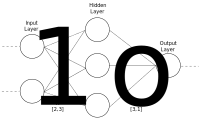
\includegraphics[width=.8\textwidth]{figures/neuralnetwork.pdf}
    \caption[Neural network example]{A simple schematic of a neural network. Each circle represents a neuron, the solid arrows represent connections between neurons, and the dotted arrows represent input and output channels. The dimensions of the network parameters are denoted as $W_n$, where $n$ refers to the output layer of the parameters. This network speifically is a fully connected feedforward \acrlong{ann} with one hidden layer. }
    \label{fig:neuralnetwork}
\end{figure}

The activation function, also known as the transfer function, is denoted as $\sigma$. Its purpose is to bound the value of a neuron so that the network is not crippled by divergent neurons \cite[81]{Wang2003}. There are many different activation functions, and some examples are presented in \cref{tab:activationfunctions} and plotted in \cref{fig:activationfunctions}. Furthermore, the activation function is used to introduce nonlinearity to the network\footnote{For this reason, the identity activation function $f(x)=x$ generally performs poorly.}, and it can be shown that a two-layer deep neural network with a nonlinear activation function is a universal function approximator \cite{Cybenko1989}. 

\begin{table}[htbp]
    \centering
    \caption[Activation functions]{Overview of some of the commonly used activation functions in neural networks. }
    \label{tab:activationfunctions}
    \begin{tabular}{ll}
    \hline
    Name & Function, $f(x)$ \\
    \hhline{==}
    Identity & $x$ \\
    Rectified Linear Unit (ReLU) & $\max\left(0, x\right)$ \\
    Leaky Rectified Linear Unit (LReLU) & $\max\left(\alpha x, x\right), \alpha\in[0,1]$ \\
    Logistic/soft step & $\frac{1}{1+e^{-x}}$  \\
    tanh & $\frac{e^x - e^{-x}}{e^x + e^{-x}}$ \\
    Softplus & $\ln\left(1+e^x\right)$ \\
    \hline
    \end{tabular}
\end{table}

\begin{figure}[htbp]  
    \centering
    \includegraphics[width=.8\textwidth]{figures/activationfunctions.pdf}
    \caption[Activation functions]{Plot showing a selection of activation functions for $x\in[-2,2]$. Note that identity, ReLU, and LReLU are overlapping for $x\in[0,-2]$. }
    \label{fig:activationfunctions}
\end{figure}
\todo[]{Change order of activation functions to be same in table and plot. }

The output of a neural network can be defined to be any shape. Depicted in \cref{fig:neuralnetwork} the output is a singular value, however it could just as well have been defined as a vector of two values. If the output is a singular value it can for instance be interpreted as a probability, however if it is a vector of length $n$ it can be seen as $n$ probabilites of different events or features. The output of a neural network is often called a feature map, because it can be seen as a mapping of the features of the input data. 

As an example, if a neural network is trained with a dataset containing images of handwritten digits $0-9$, an output with a size of $10$ could contain probabilities of a given image containing a specific digit where each output value is the probability of one digit. One well-known dataset that is often used for this exact problem is the MNIST dataset \cite{mnist}.


\section{Neural Network Types}
There are many different types of neural networks that are suited for different problems. Here, a selection of types that lead up to the \acrfull{gan} structure used in this thesis will be introduced. 

\subsection{Artificial Neural Network}
The \acrfull{ann} is the simplest type of a neural network, and it is the architecture that was described in \cref{sec:ml:componentsofaneuralnetwork}. It consists of neurons that build up layers. A simple example of a fully connected feedforward \acrshort{ann} can be seen in \cref{fig:neuralnetwork}. 

% Affine transformations and pointwise nonlinearities which are smooth Lipschitz functions (such as sigmoid, tanh, elu, softplus, etc.). 

\subsection{Convolutional Neural Network}
A \acrfull{cnn} builds upon the structure of the \acrshort{ann}, however it adds a new type of layer: the convolutional layer. Instead of containing a set of neurons, this layer contains one (or more) convolutional kernel(s), and performs a convolution of the input to the layer with the kernel(s). This type of network was first introduced in \citeyear{lecun1999object}, and has shown to work very well for many different image related tasks \cite{lecun1999object,alexnet}. Because of the nature of the convolutions, it allows the network to utilize 2D information by performing 2D convolutions\footnote{Likewise higher-dimensional information may be used by performing higher-dimensional convolutions \cite{8353466}}. This has been shown to perform exceptionally well in image processing tasks \cite{alexnet,oshea2015introduction}. 

% Reduce number of trainable parameters, zero-padding, kernel size, stride, number of kernels per layer
\todo[inline]{More on convolution}
\missingfigure{Convolution visualisation}

\subsection{Encoder-Decoder Network}
Downscaling and upscaling between layers, and skip connections (for U-net, but not actually in encoder-decoder networks). % https://www.researchgate.net/post/Are_U-net_and_encoder-decoder_network_the_same 

\subsection{Generative Adversarial Network}
Learn probability distribution and generate random sample from learned distribution. 
GAN based on game theory instead of optimization. \cite{goodfellow2014gan,goodfellow2020gan}. 

\section{Training a Neural Network}
The process of tuning all the parameters (i.e. weights and biases) of a neural network is called training. During training, input data from a training dataset is forwards propagated through the network, and the resulting feature map is compared to an expected feature map (e.g. manually labeled data)\footnote{This is what is called supervised learning, as opposed to unsupervised learning where there is no ground truth answer to compare to. }. The difference in these feature maps is calcuated using some loss function, and the loss is then backwards propagated through the network to update each and every parameter to reduce the loss. 

Generally, the entire training dataset is repeatedly passed through the network multiple times. Each full runthrough of the training dataset is called an epoch of training. This however can often introduce a problem: the training dataset can typically not fully fit in the computer memory at once. Therefore it is divided into mini batches, and after each mini batch the weights are adjusted. The propagation of one mini batch is often called one iteration, and thus one epoch consists of several iterations. The size of a mini batch is a tunable parameter, however typically it is in the range of $32-512$ (e.g. 128 in the well-known article by A. Krizhevsky et al. \cite{alexnet})\footnote{There is ongoing research into techniques to increase the batch size by several orders of magnitude as larger batches allow for easier parallelization, however large batch sizes have been shown to cause instability during training \cite{you2017large}. }. The size of a mini batch can sometimes also be refered to as the batch size. 

\subsection{Hyperparameters}
During training, the parameters of the neural network are automatically changed, however there are some parameters that are set manually beforehand. These are called hyperparameters \cite{claesen2015hyperparameter}. Some typical hyperparameters are:
\begin{itemize}
    \item Number of layers (i.e. depth of network).
    \item Size of layers.
    \item Learning rate.
    \item Number of iterations to train the network (i.e. number of epochs).
    \item Mini batch size.
\end{itemize}

The process of choosing these hyperparameters is not an exact science, and there is research being done into finding ways of automatically tuning hyperparameters to their ideal configurations, called auto-tuning \cite{autotuning}.

\subsection{Loss Functions}
To properly quantify the error, or loss, of a neural network one needs to define some metric. These are called loss functions. Depending on the problem type, diferent loss functions may perform better than others, however there are some standard loss functions often used. Some of these as well as some specific ones used in this thesis will be presented here.

Perhaps the most commonly used loss function is the \acrfull{mse}. It is closely related to the L2-norm, and it can be defined as
\begin{equation}
    \label{eq:mse}
    L_{\text{MSE}} = \frac{1}{N} \sum_{i=1}^N(Y_i - \hat{Y}_i)^2,
\end{equation}
where $Y$ is the correct (labeled) value and $\hat{Y}$ is the predicted value. This often performs well, however in cases such as image processing or image superresolution it has shown to cause blurring \cite{7797130}.

Another similar loss function is the \acrfull{mae}, which is closely related to the L1-norm. It can be defined as
\begin{equation}
    \label{eq:mae}
    L_{\text{MAE}} = \frac{1}{N} \sum_{i=1}^N |Y_i - \hat{Y}_i|,
\end{equation}
with $Y$ and $\hat{Y}_i$ being the same as previously defined. This loss function does not over-penalize larger errors, and therefore may have different convergence properties than \acrshort{mse} \cite{7797130}. It has been shown to perform better than \acrshort{mse} in some image processing cases \cite{7797130,10.1002/mp.13713}.

A more recently introduced loss function is the log-cosh loss function, defined as \cite{chen2019log}
\begin{equation}
    \label{eq:logcosh}
    L_{\text{Log-cosh}} = \frac{1}{a} \sum_{i=1}^N \log ( \cosh ( a ( Y_i - \hat{Y}_i))),
\end{equation}
where $Y$ and $\hat{Y}$ are as previously defined, $\log$ is the logarithm, $\cosh$ is the hyperbolic cosine function, and $a$ is some positive hyperparameter $a \in \mathbb{R}^+$. It behaves similar to \acrshort{mse} around the origin, and similar to \acrshort{mae} at other points. It has been shown to perform well in image processing related tasks \cite{7797130}.
% MSE, MAE, LogCosh, VGG, Adversarial

All the aforementioned loss functions rely on pixel-wise losses. Another type of loss functions that has shown to perform well in image processing related tasks is the use of a feature space based loss \cite{vggloss}. Specifically, this loss is based on measuring the difference in the feature space of the inferrence of a pre-trained network. Here, the pre-trained VGG network is used to measure a visual loss \cite{simonyan2015deep}. This specific loss function is termed visual loss, or VGG loss, and is defined as \cite{vggloss,liu2020tomogan}
\begin{equation}
    \label{eq:vgg}
    L_{\text{VGG}} = \sum_{i=1}^{N} \sum_{j=1}^{W_f} \sum_{k=1}^{H_f} \left(V_{\theta_{\text{VGG}}} (Y_i)_{j,k} - V_{\theta_{\text{VGG}}} (\hat{Y}_i)_{j,k} \right)^2,
\end{equation}
where $Y$ and $\hat{Y}$ are as previously defined, $V_{\theta_{\text{VGG}}}(Y)$ is the VGG feature map representation of image $Y$, and $W_f$ and $H_f$ are the dimensions of the feature maps extracted by the pre-trained VGG network. The VGG network is trained with natural images, specifically the ImageNet dataset \cite{deng2009imagenet}, however it has been shown to work well as a feature extractor for \acrshort{ct} images \cite{8340157}. 

\todo[inline]{Adversarial loss}

\subsubsection{Weighted loss}
In practise it is common to use a weighted sum of different loss functions. 
An example containing \acrshort{mse}, log-cosh, and VGG loss can be given as
\begin{equation}
    \label{eq:weightedloss}
    L_{\text{Total}} = \lambda_{\text{MSE}}L_{\text{MSE}} + \lambda_{\text{Log-cosh}}L_{\text{Log-cosh}} + \lambda_{\text{VGG}}L_{\text{VGG}},
\end{equation}
where $\lambda_N$ is a hyperparameter controlling the weight of $L_N$. 

\subsection{Backpropagation}


\subsection{Optimizers}

\subsubsection{Stochastic Gradient Descent}
Article: \cite{stochasticgradientdescent}

\subsubsection{ADAM}
Article: \cite{kingma2015adam}

\chapter{Method and Datasets}
\label{sec:method}

\section{TomoGAN}
GAN where input is not random, but noisy image. U-net structure (encoder-decoder). Extract feature map of noisy image where noise is removed, and generate image from noiseless feature map. 
TomoGAN \cite{liu2020tomogan}


\section{Datasets}
\subsection{TomoBank}
TomoBank \cite{TomoBank}

Tomopy \cite{tomopy}.

Making a dataset: scaling, cropping, sorting, selecting only good images (e.g. ignore empty from top of stack). 

\subsection{In-house}
ASM\_ID16B\_phaseContrast\_Shale\_2018, 

Kim-Robert
\chapter{Results and Discussion}
\label{sec:results}

\section{Effect of Pre-processing Images}
\todo[inline]{Compare tomo\_00058 denoising with and without cropping. Without cropping similar results to early stages of denoising cropped (i.e. poor and not converged). }

\section{Hyperparameter and Loss Function Changes}
\todo[inline]{Show difference in tomo\_00058 denoising for different loss functions / weights (and hyperparameters?)}

\todo[inline]{Line plot of gt, ns, MSE denoising, Log-cosh denoising. Multiple lines around the images?}

\todo[inline]{SSIM and MSE evolution of arbitrary slice. }

\section{Different Amounts of Noise}
\todo[inline]{Different levels of noise / projection subsamplings (8,16,32,48). }
\todo[inline]{Plot of the images with zoomed in ROIs. }
\todo[inline]{Plot showing improvement in SSIM for different levels of noise. }
\todo[inline]{Line plot for different levels of noise? }

\section{Loss Function Evolution}
\todo[inline]{Plot how loss functions evolve through training of tomo\_00058 with good hyperparameters. }

\section{TomoGAN Compared to PICCS}
\todo[]{Change section name?}
\todo[inline]{Axial, sagittal, coronal plots for different depth parameters. }
\todo[inline]{Maybe make 3D model plot of this dataset. }
\todo[inline]{Line plot comparing GT, FDK?, PICCS, denoised. }
\todo[inline]{Histogram. Looks like peaks roughly align, sharper peaks. Looks like it is performing segmentation? }
\todo[inline]{}

\section{Attempted Shale Denoising}
\todo[inline]{Include this?}
\todo[inline]{Shows limitations of method: requires a high-quality similar dataset (i.e. some ground truth) to work properly. Any given trained network doesn't work for all other dataset. }

Plot types: 
\begin{itemize}
    \item \acrshort{ssim} and \acrshort{mse} changes during training.
    \item Loss function evolution.
    \item Line plot of gt, ns, and different loss functions?
    \item Histograms of gt, ns, denoised
    \item Zoomed in region of interest.
    \item Axial, sagittal, and coronal plots of (at least Kim Robert's dataset) different depth parameters.
    \item Compare denoising of different subsamplings (8, 16, 32, 48)
    \item Activation plot of network layers.
\end{itemize}
\chapter{Conclusion}
\label{sec:conclusion}
In this thesis, \gls{ct} images have been denoised using the TomoGAN denoising neural network. TomoGAN is able to achieve vast improvements in image quality for cases where a corresponding high-quality dataset is available to train the network on. 

A change to the loss function used to train TomoGAN, namely including a log-cosh loss term, was proposed and tested. It yielded minor improvements to the achieved SSIM score for denoising without introducing any discernible drawbacks. 

The 3D denoising capabilities of TomoGAN have been explored. The use of the depth parameter of TomoGAN allows the denoising to utilize 3D spatial information when denoising, reducing the interaxial artifacting introduced by denoising single axial slices of a 3D object. Denoising of a dynamic \gls{ct} dataset imaging soda lime glass spheres achieves comparable image quality to \gls{piccs} based reconstruction. 

The method is highly dependent on having access to good training data. For denoising where there is no available dataset to train the network, the method is unable to produce usable denoisings. This method is therefore not suited for general-purpose denoising of arbitrary datasets.

Furthermore, the network has been shown to require the training data to be pre-processed to a suitable format in order to achieve usable results. 


\section{Further Work}
When 3D datasets are denoised, the TomoGAN denoising neural network is only able to capture 3D information through the use of the depth parameter. The transformation from noisy to noiseless images itself is a 2D transformation (through the use of 2D convolutions). Implementing the same network with 3D convolutions to truly be a 3D denoising method may yield vast improvements to the results. \Gls{ct} imaging is a 3D technique, and the denoising method should utilize that fact.

Furthermore, altering the structure of the network has not been explored in this thesis. The field of \glspl{gan} is in rapid development, and altering the structure of the generator in TomoGAN to utilize new discoveries that may arise, may further improve results. 

Image augmentation (e.g. rotation, zoom, flips) may be used to increase the size of the training dataset in situations where a limited training dataset is available, however this will still require access to a suitable training dataset for a given noisy dataset. Unfortunately, this is a limitation of this method. 

There is no inherent feature of TomoGAN currently making it only usable for \gls{ct} images. When the depth parameter is unused, it is merely performing image-to-image translation. Some other denoising techniques use the Radon transform to include the reconstruction process itself in the denoising. Altering the TomoGAN method to utilize the full extent of the information available from \gls{ct} imaging (e.g. a sinogram-based loss) may further improve the method. 

% NOTES:

% Cross-entropy:
% https://towardsdatascience.com/understanding-binary-cross-entropy-log-loss-a-visual-explanation-a3ac6025181a



\chapter*{\bibname}
\printbibliography[heading=none]


\appendix

\end{document}
